% Chapters content

\chapter{Introduction}

\section{Context}

For several years, Carl Haber and his team at Lawrence Berkeley National Laboratory (\gls{lbnl}) have been working on the sound recovery of old mechanical records. They developed two different systems able to extract the sound without any physical contact, using optical methods. These are capable to process many different types of mediums, from early Edison records to vinyl discs, including shellac or lacquer composed discs and others.

Nowadays, a lot of unique and historical records remain in archives from different libraries and museums. They contain some important historical and cultural recordings but as they are aging and deteriorated, it is too delicate to play them with a normal mechanical phonograph. Non-contact feature of optical methods is then important.

The first developed system is called \gls{irene}. It enables to extract the sound using digitized images of the disc. The corresponding program that processes the extraction from the acquisition step is called \gls{rene}.

The second one, \gls{3dprobe}, uses a special probe able to measure the real depth at each position of the scanned record. This gives the best results for certain types of records as the cylinders.

Meanwhile in Switzerland, at the College of Engineering and Architecture of Fribourg, a project called VisualAudio has been developed. It also enables to extract the sound using non-contact optical scanning in a similar manner as \gls{irene}, but it does not apply to experimental records such as cylinders.

\section{Project goals}

Old records can suffer from degradations. One of the most common is known as ``cracked discs''. This problem appears when the lacquer coating shrinks as the disk is getting older. This causes cracks where the underneath hard support is visible, as seen in \autoref{fig:crackeddisc}.

\begin{figure}[!ht]
\centering
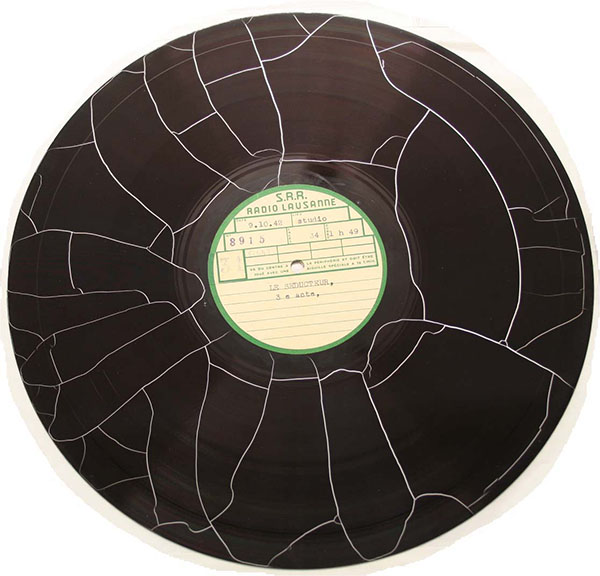
\includegraphics[width=0.7\textwidth]{images/cracked-disc}
\caption{An example of cracked disc.}
\label{fig:crackeddisc}
\end{figure}

Up to now, \gls{irene} and \gls{3dprobe} cannot automatically process such damaged records, because the groove traces are sometimes widely separated and may be shifted from each other. Though a special feature is implemented, enabling the user to manually track the traces, it is not a perfect tool for practical use. Moreover, even with such a feature, it could be really difficult to visually find the correct shifting when the traces look similar.

The aim of this Master's thesis is to find ways to read correctly these kinds of degraded records with the solutions developed at LBNL by Carl Haber and his team. In a first step, an improvement of the manual tracking will be implemented. It is still useful to keep it for some cases, e.g for special early recordings or when a disc is heavily cracked.

Then, the next step will be to design and implement a tracking feature able to process cracked records and link their traces automatically. VisualAudio already implements such a feature. It can then be taken as an example, though it is obviously not possible to directly use its implementation, due to the differences between the systems.

%\section{Report structure}

%TODO This report is separated in...

\chapter{Phonograph cylinders and records}

This chapter will give a quick historical overview of the different mechanical phonograph technologies and the types of mediums encountered. It will also explain the main principles behind the analog recording

\section{History}

The first known sound recording was realized by the French printer Édouard-Léon Scott de Martinville in 1860. However, the used device called the \emph{phonautograph} was not able to playback the recordings. It acted as an early oscilloscope and was used by scientists to study visual representations of the sound.

The phonograph was created by Thomas Edison in 1877. It was the first device able to record \emph{and} reproduce the sound. The general principle was to mechanically engrave the audio signal on a rotating cylinder. The resulting groove undulated then vertically. Then, for the playback, a stylus (needle) retraced the groove and was able to reproduce the sound waves from the generated vibrations. Finally, the signal was amplified with a horn so that the recording was audible. A newer version of this phonograph and an example of cylinder are presented in \autoref{fig:edisonphonocyl}.

\begin{figure}[!ht]
    \begin{subfigure}[b]{0.49\textwidth}
    \centering
    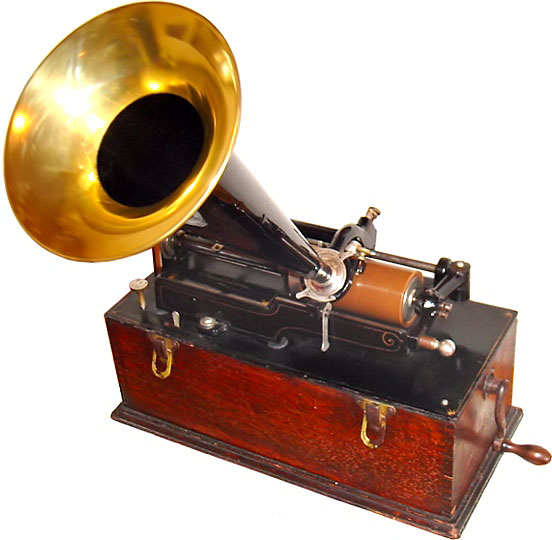
\includegraphics[height=0.5\textwidth]{images/edison-phonograph}
    \caption{An Edison phonograph.}
    \label{fig:edisonphono}
    \end{subfigure}
    \begin{subfigure}[b]{0.49\textwidth}
    \centering
    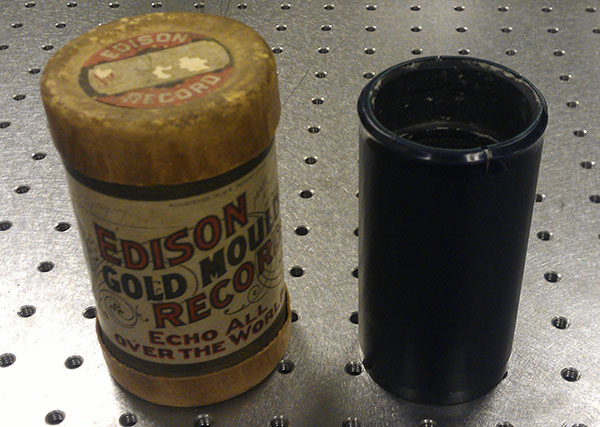
\includegraphics[height=0.5\textwidth]{images/edison-cylinder}
    \caption{An Edison wax-cylinder.}
    \label{fig:edisoncyl}
    \end{subfigure}
    \caption{Pictures of Edison wax phonograph and record.}
    \label{fig:edisonphonocyl}
    %\floatfoot{Norman Bruderhofer, www.cylinder.de}
\end{figure}

Since then, the phonograph has been used as the only device for sound reproduction until around the 1950's when the magnetic tape has become widely used on the market. From the first Edison's version, a lot of improvements have been made. Edison used first a tinfoil around the cylinders to engrave the groove. However, this material gave bad quality and was rapidly degrading. Alexander Graham Bell started to use wax-coated cylinders instead of the tinfoil, which improved a lot the sound quality.

Then, in the early twentieth century, the cylinders were gradually replaced by the gramophone records which were flat discs that could be double-sided. On the latter, the groove undulated laterally instead of vertically.

After the wax-cylinders, a lot of different materials have been used for the discs covering. For example, the shellac discs became the first widely used medium. Some discs were also using a special lacquer coat. Finally, the vinyl disc is one of the last types of gramophone record and is still being used today.

\section{Basic principle}

\subsection{Edison phonograph}

With the early Edison phonograph, the same device was used to record and replay the sound. As already explained, the sound is mechanically engraved with a needle. In fact, the needle is connected to a diaphragm that vibrates when audio waves are emitted. The cylinder is put on a mechanism which can be rotated by a crank and that shifts slowly resulting in helical grooves, as represented in \autoref{fig:phonoschema}.

\begin{figure}[!ht]
\centering
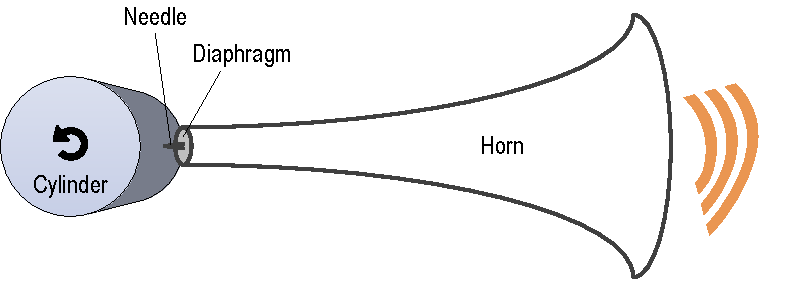
\includegraphics[width=0.9\textwidth]{images/phono-schema}
\caption{Schema of a simple phonograph.}
\label{fig:phonoschema}
\end{figure}

Then, to reproduce the recorded sound, the cylinder is repositioned at its starting position. The needle is placed with slightly less pressure, and when the crank is turned, the needle follows the groove which vibrates the diaphragm and returns the sound waves. This is in fact the exactly inverse process as the recording.

\subsection{Other recording types}

The Edison phonograph uses a groove that undulates vertically. However, a lot of records, particularly the discs, have used laterally modulated grooves. This way, it is no more the depth that determines the signal, but rather the lateral position of the bottom of the groove. The difference can be clearly seen in \autoref{fig:groovesdiff}.

\begin{figure}[!ht]
    \begin{subfigure}[b]{0.49\textwidth}
    \centering
    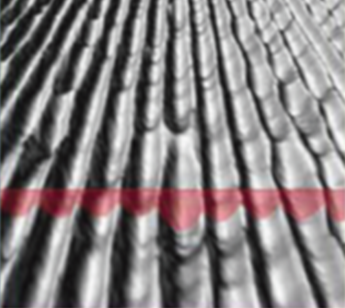
\includegraphics[width=0.8\textwidth]{images/grooves-vertical}
    \caption{Vertically modulated.}
    \label{fig:groovesvert}
    \end{subfigure}
    \begin{subfigure}[b]{0.49\textwidth}
    \centering
    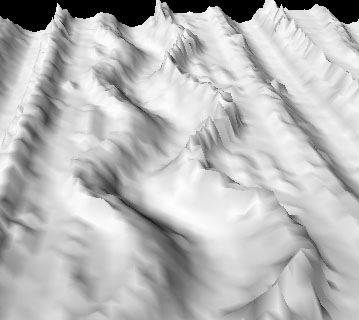
\includegraphics[width=0.8\textwidth]{images/grooves-lateral}
    \caption{Laterally modulated.}
    \label{fig:grooveslat}
    \end{subfigure}
    \caption{The two types of groove modulation.}
    \label{fig:groovesdiff}
    %\floatfoot{Norman Bruderhofer, www.cylinder.de}
\end{figure}

It exhibits a 3D representation of record surfaces for both groove types. In \autoref{fig:groovesvert} the boundaries are straight and the depth  varies while in \autoref{fig:grooveslat} they form an horizontal wave.

\section{Summary}

This chapter gives an idea of the phonograph history and different devices, showing the heterogeneous nature of the audio recording, with a lot of different techniques and materials. This outlines the difficulties that might appear while trying to recover old recordings.

\chapter{Acquisition and processing systems}

This chapter will detail the systems used in the audio laboratory at LBNL to extract records. For both systems, the main process is separated in two main steps: the acquisition and the processing.

\section{IRENE}

\subsection{Acquisition}

As already explained, \gls{irene} uses numerical macro photography for the acquisition. The scanner takes some monochromatic pictures of the disc. The resulting image is influenced by the shape of the surface because of the light reflection. Therefore, the intensity of the resulting pixels depends finally on the slope at this of the surface light reflection.

%This enables to visually find the grooves on the resulting picture. An example of such a picture is shown in xx.

%In fact, the camera cannot take a whole picture of one disc in a snapshot.  yy shows the image zoomed out of 

\section{PRISM}

%TODO

%\chapter{Sample recordings}

%TODO???.

%\chapter{Manual tracking}

%TODO.

%\section{Design}

%TODO.

%\section{Implementation}

%TODO.

%\chapter{Automatic scanning}

%TODO.

%\section{Design}

%TODO.

%\section{Implementation}

%TODO.

%\chapter{Tests and extraction of the sample recordings}
%
%TODO.

%\chapter{Conclusion}
%
%TODO.

%------------------------ Float samples ------------------------

%\begin{figure}[!ht]
%\centering
%
\includegraphics[width=0.7\textwidth]{images/logo_lbnl}
%\caption{Image caption.}
%\label{fig:figname}
%\end{figure}

%\begin{table}[!ht]
%\begin{center}
%\begin{tabular}{| l c r |}
%    \hline
%    1 & 2 & 3 \\
%    4 & 5 & 6 \\
%    7 & 8 & 9 \\
%    \hline
%\end{center}
%\end{table}

%\begin{lstlisting}[language=C++, caption={Test listing}, label={lst:listingname}]
%// Comment
%int i;
%char c;
%\end{lstlisting}

%\autoref{eq:solve} with variable $s$ such as:
%\begin{equation} \label{eq:solve}
%s = [a_0, (a_0 + a_1), ..., (a_0 + a_1 + ... + a_{n-1})].
%\end{equation}
